\documentclass{article}
\documentclass[a4paper,12pt]{article}
\usepackage[english]{babel}
\usepackage[utf8]{inputenc}
\usepackage{amsfonts}
\usepackage{indentfirst}
\usepackage[T1]{fontenc}
\usepackage{amsmath}
\usepackage{hyperref}
\usepackage{graphicx}
\usepackage{subfig}
\usepackage[export]{adjustbox}

\textwidth\paperwidth
\advance\textwidth -45mm
\oddsidemargin 18mm
\advance\oddsidemargin -18mm
\evensidemargin 18mm
\advance\evensidemargin -18mm
\topmargin -30mm
\advance\topmargin 17mm
\setlength\textheight{45\baselineskip}
\addtolength\textheight{\topskip}
\marginparwidth 15mm


\title{
\textbf{Human Recognition by Biometric Methods}\\
\bigskip
\textbf{Face detection and classification}\\
\bigskip
}
\author{Mikołaj Małkiński}
\date{7 June 2018}

\begin{document}

    \maketitle

    \section{Description of the assignment}\label{sec:descriptionOfTheAssignment}

    The goal of this task was to design, implement and train YOLO object detection system for detecting faces of Polish rappers.
    Then, the extracted face should be piped to previously trained model in order to classify it.

    The original dataset defined around 700 hundred bounding boxes for faces.
    Several boxes could refer to the same image.
    The dataset was split automatically into two parts by Keras, using 80\% of the data for training and remaining 20\% for validation.

    The models are resizing the images before processing, so data of arbitrary size can be used.
    However, it is important to note that images have to be in the same format (\textit{jpg} used in this case).
    Therefore, part of the preprocessing involves converting images from \textit{png} format to \textit{jpg}.
    Lack of this conversion caused unbearable accuracy - close to 0\%.

    The project conists of following scripts:
    \begin{itemize}
        \item $evaluate$ - evaluates model accuracy and loss on specified dataset,
        \item $predict$ - predicts a class of specified image,
        \item $reproduce\_results$ - creates plots shown in the report,
        \item $train$ - trains given model on specified dataset.
    \end{itemize}

    \section{Analysis of results}\label{sec:analysisOfResults}


    \section{Hyperparameters}\label{sec:hyperparameters}

    Figure~\ref{fig:compare1} presents comparison between two configurations described in the Figure~\ref{fig:configurations1}.
    \begin{figure}[!h]
        \centering
        \begin{tabular}{cccc}
            \textbf{Configuration} & \textbf{Min input size} & \textbf{Max input size} & \textbf{Batch size} \\
            1 & 128 & 288 & 4 \\
            2 & 288 & 448 & 2
        \end{tabular}
        \caption{Details of configurations}
        \label{fig:configurations1}
    \end{figure}

    \begin{figure}[!h]
        \centering
        \begin{tabular}{cc}
            \subfloat[Loss]{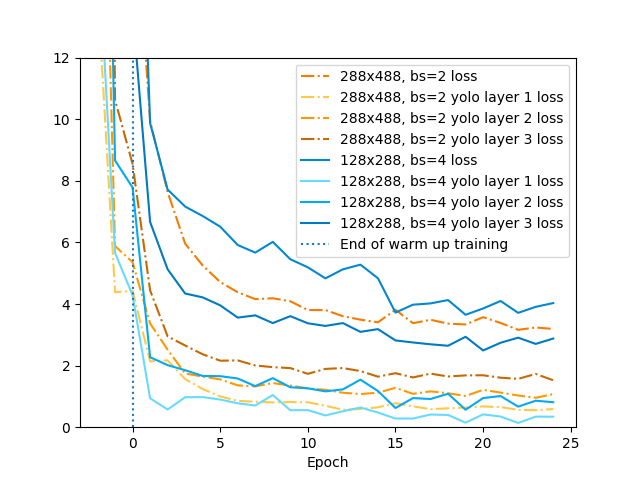
\includegraphics[width = 0.5\textwidth]{plots/compare_loss_face_01_06_15-25-face_05_06_15-08.png}} &
            \subfloat[Mean Average Precision at 0.5]{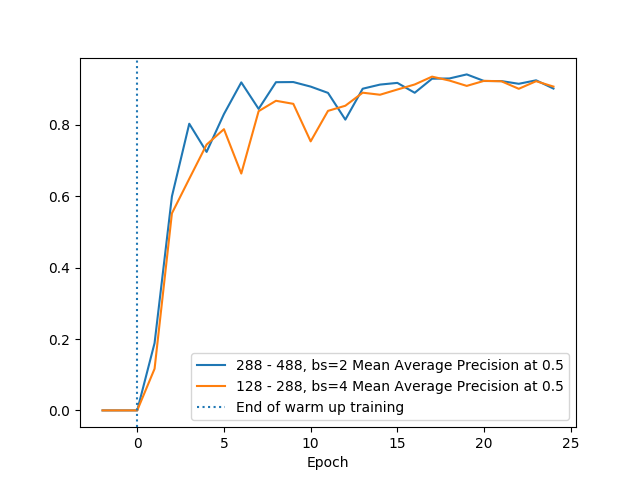
\includegraphics[width = 0.5\textwidth]{plots/compare_map_face_01_06_15-25-face_05_06_15-08.png}} \\
        \end{tabular}
        \caption{Comparison of two configurations}
        \label{fig:compare1}
    \end{figure}

    \subsection{Batch size}\label{subsec:batchSize}
    Batch size is one of the hyperparameters which can influence the network accuracy.
    During experiments, two batch sizes were analysed: 16 and 32.
    Unfortunately, starting from 64, the batch of images was too big to fit it into GPU memory.
    In the Figure~\ref{fig:vgg16_bs_compare} the influence of mentioned batch sizes are shown.
    It can be noticed, that larger batch size gave slightly better results, but the difference isn't huge.

    \newpage
    \section{Analysis of predictions}\label{sec:analysisOfPredictions}
    In the Figure~\ref{fig:wrong_predictions} some of wrong predictions of fine-tuned version of VGG16 are shown. Finally, Figure \ref{fig:confusion_matrix} presents the confusion matrix of mentioned network.


\end{document}
